% !TeX TS-program = txs:///duck
% Created by Denis Bitouzé 
% https://texnique.fr/osqa/questions/7046/mettre-un-paragraphe-de-texte-et-une-image-cote-a-cote/7055
\documentclass{standalone}

\usepackage{tikzducks}

\begin{document}

  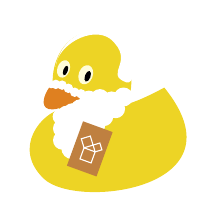
\begin{tikzpicture}
    \duck[recedinghair=white,beard,book]
    \begin{scope}[scale=0.03,rotate=-20,xshift=500,yshift=700]
    \draw[white,rotate around={36.9:(5,5)}] (5,5) rectangle ++(3,3);
    \draw[white,rotate around={36.9:(0,5)}] (0,5) rectangle ++(4,4);
    \draw[white] (0,0) rectangle (5,5);
    \end{scope}
  \end{tikzpicture}
  
\end{document}